\subsection{Stroj in OS}

\subsection{Testni primeri}

V tem poglavju je opisana empirična primerjava časovnih zahtevnosti različnih operacij, poizvedb in izgradnje ter prostorske zahtevnosti različnih implementacij priponskega drevesa. Priponsko drevo se uporablja za iskanje vzorcev v besedilu $T$, torej se je smiselno osredotočiti zgolj na primerjavo časovnih zahtevnosti za poizvedbe ter za izgradnjo priponskega drevesa. Primerjava posamičnih operacij priponskega drevesa nima smisla, saj se le te uporabljajo pri implementaciji poizvedb in izgradnji. 

Pri tem se bomo osredotočili zgolj na osnovne poizvedbe. Kot najbolj preprosta osnovna operacija bo izdelana primerjava nad poizvedbo $prisotnos(vzorec)$. Ta poizvedba je bila izbrana, saj je pogosto vprašanje v biologiji prisotnost genov (vzorcev) v DNK sekvenci, ne pa natančen položaj tega gena ali števila ponovitev vzorca. Čas izvajanja poizvedbe bo izmerjen kot razlika v času takoj pred začetkom izvajanja poizvedbe ter takoj po zaključku izvajanja poizvedbe. Poizvedba bo izmerjena na vzorcih dolžine 5 znakov, 50 znakov, 500 znakov in $\log{n}$ znakov, kjer je $n$ dolžina znaka. 

Na podoben način kot poizvedba $prisotnos(vzorec)$ bo izmerjen tudi čas izgradnje priponskega drevesa. Le ta bo izmerjen s pomočjo razlike v uri med časom ure takoj pred izgradnjo ter v časom ure takoj po izgradnji priponskega drevesa.

Izmerjeni časi bodo shranjeni v vektorju potrebnih časov $T_{i,v}$, pri čemer $i$ predstavlja dolžino vhodnega besedila in $v$ predstavlja tip priponskega drevesa (priponsko drevo z vrednostjo $v=ST$ ali kompaktno priponsko drevo z vrednostjo $v=CST$). Vektor bo sestavljen na sledeči način
\begin{equation*}
    T_{i,v}=(t_{izg},t_5,t_{50},t_{500},t_{\log{n}}),
\end{equation*}
pri čemer so izmerjeni časi za poizvedbe izmerjeni v nanosekundah, čas izgradnje $t_{izg}$ pa v milisekundah. 

Na podoben način bo shranjena tudi velikost, ki jo zasede priponsko drevo v delovnem spominu. Izmerjen prostor bo poleg prostora priponskega drevesa vseboval tudi besedilo $B_{0}$, katerega podniz $B_0[1,i]$ bo uporabljen za izgradnjo. Ker bodo vse meritve vsebovale velikost besedila $B_0$, le to ne bo vplivalo na primerjavo podatkov. Izmerjen prostor bo shranjen v vektorju $S_{i,v}$, pri čemer $i$ predstavlja dolžino vhodnega besedila in $v$ predstavlja tip priponskega drevesa (priponsko drevo z vrednostjo $v=ST$ ali kompaktno priponsko drevo z vrednostjo $v=CST$). V tem primeru bo vektor $S_{i,v}$ vseboval zgolj vrednost $s_{max}$, ki je največja dosežena velikost priponskega drevesa med izvajanjem izgradnje in poizvedbe. Največji izmerjeni zasedeni prostor na delovnem spominu bo izmerjen z uporabo pomnilniškega profilerja (angl. \textit{memory profiler}).

Uporabljeni bo Bytehound \cite{Bytehound2024} pomnilniški profiler, saj omogoča grafični prikaz porabe spomina v času izvajanja programa. Primer prikaza porabe delovnega spomina v času izvajanja testa je prikazan na Sliki \ref{fig:ZasedonestRAM}. Na sliki se jasno vidi, da večanje priponskega drevesa povzroči rast zasedenega prostor na delovnem spominu v času izgradnje in poizvedbe. Na sliki se lahko opazi, da izgradnja in poizvedbe v kompaktnem priponskem drevesu potrebujejo krepko manj časa in prostora, zato izgleda, kot da se graf konča malo pred koncem vodoravne osi. Razlog za to je izgradnja in poizvedba nad kompaktnim priponskim drevesom, ki potrebuje manj pomnilnika in posledično manj časa za dodeliti in sprostiti delovni spomin.

\begin{figure}[tb]
    \begin{center}
        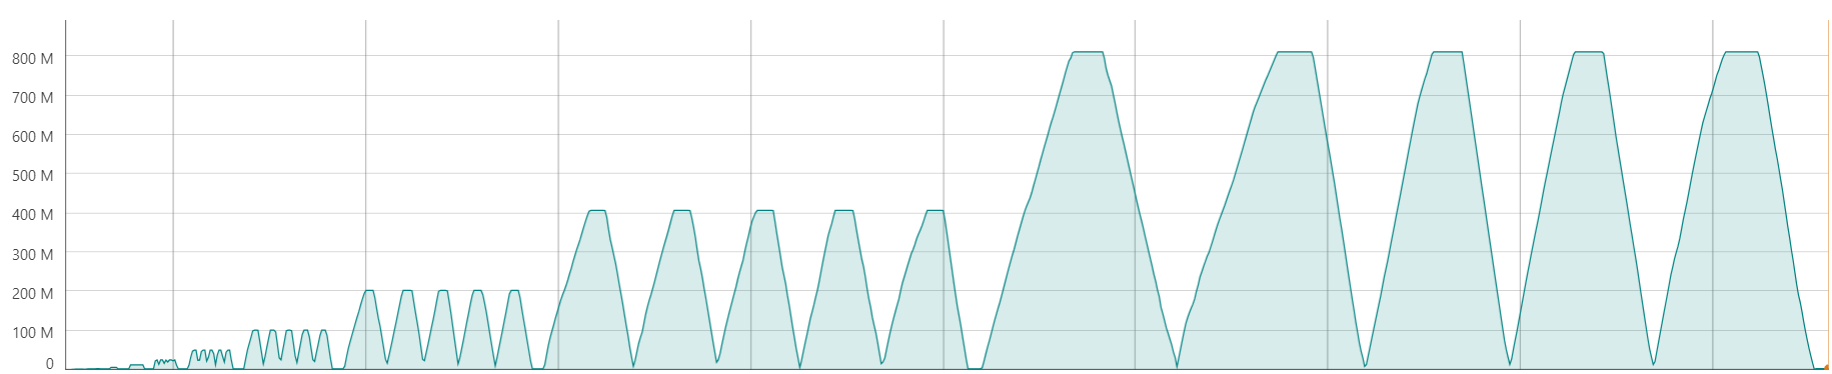
\includegraphics[width=\textwidth]{Slike/bytehoundGraf.png}    
        \captionof{figure}[Zasedenost spomina testiranjem različnih implementacij priponskega drevesa skozi celotno izvajanje testa.]{Zasedenost spomina testiranjem različnih implementacij priponskega drevesa skozi celotno izvajanje testa.} 
        \label{fig:ZasedonestRAM}    
    \end{center}
\end{figure}


Za zmanjšati vpliv ostalih procesov na računalniku, se je vsak test ponovil 5-krat. To je tudi vidno na Sliki \ref{fig:ZasedonestRAM}, zato ima zadnje izgrajeno prionsko drevo 5 vrhov in vsak vrh predstavlja eno ponovitev testiranja. S pomočjo profilerja je bila tudi izmerjena velikost originalnega besedila $B_0$, ki je prikazan v zadnjem stolpcu Tabele \ref{tab:besedila}, saj se velikost razlikuje glede na vhodno besedilo.

\begin{table}[htb]
    \caption{Primerjava besedil, ki bodo uporabljena za primerjavo različnih implementacij priponskih dreves}
    \label{tab:besedila}
    \centering
    \begin{tabular}{rccc}
        Ime testnega besedila& Število znakov & Velikost abecede & Velikost na disku \\
        &  &   & [MB]\\
         \hline
        Ivan Cankar, Na klancu \cite{podatkiNaKlancu}& 317803 & 52 & $25,851$ \\
        DNK sekvenca \cite{podatki}&  52428800& 4 & $26,767$ \\
    \end{tabular}
    
\end{table}

S tem načinom testiranja se želita ugotoviti dve stvari. Najprej se želi ugotoviti vpliv velikosti vhodnega besedila na čas izgradnje in poizvedb nad priponskim drevesom ter velikost spomina, ki ga zasede priponsko drevo. To bo izmerjeno z izgradnjo različnih dreves ter s poizvedbami nad njimi. Prvo drevo bo izgrajeno nad besedilom dolžine 500 znakov. Vsako naslednje priponsko drevo bo izgrajeno nad besedilom, ki je dvakrat daljše od predhodnega. Zadnje izgrajeno priponsko drevo bo imelo dolžino besedila, za katerega je bilo izgrajeno, manjšo od $|B_0|-500$ znakov ali $|B_0|-\log{(500\cdot2^{i-1})}$ za besedila daljša od $2^{500}$ znakov. V besedilu mora bit vedno na voljo dovolj znakov, da se bodo lahko iz njih naredili vzorci vseh testiranih velikosti. Besedilo, ki bo uporabljeno za izgradnjo $i$-tega priponskega drevesa, bo podniz $B_0[1,500\cdot2^{i-1}]$.

 Druga stvar, ki se želi ugotoviti, je vpliv uporabe \verb|swap| razdelka za namene delovnega spomina ter vpliv velikosti abecede vhodnega besedila in vzorca na iskanje vzorca v priponskem drevesu. Zato bo primerjava narejena na dveh besedilih, ki imata različno vhodno abecedo, in sicer prvo vhodno besedilo je kratki roman Ivana Cankarja, Na klancu \cite{podatkiNaKlancu}, ki uporablja slovensko abecedo, ter daljša DNK sekvenca \cite{podatki}, ki pa uporablja abecedo $\Sigma = \{A,C,T,G\}$. Pri tem obe abecedi ne vsebujeta znaka, ki predstavlja konec besedila, $\$$, saj bo le ta dodan besedilu pred začetkom izgradnje. Več podatkov o vhodnih besedilih je prikazanih na Tabeli \ref{tab:besedila}.


\subsection{Pred obdelava besedil}

Kot je razvidno v drugem stolpcu Tabele \ref{tab:besedila} je potrebno najkrajše besedilo podaljšati. Ker je malo verjetno, da se vhodno besedilo ponovi $k$-krat, dokler ne doseže primerne velikosti, predvsem v naravnem jeziku, bo uporabljena bolj napredna metoda podaljševanja besedila. Metoda vzame manjše dele besedila dolžine $5i$ ter jih konkatenira na koncu besedila. Tako dobljeno besedilo je bolj verjetno, saj je večja verjetnost, da se manjši deli besedila ponovijo za razliko od celotnega besedila. Predlagana metoda podaljševanja besedila je prikazana z Algoritmom \ref{alg:Konkatenacija}. Pri tem metoda predpostavi, da je besedilo dolgo vsaj $6i$, kar je $3000$ znakov dolgo. Ta metoda je primerna za podaljševanje daljših besedil, sicer pa je možno metodi spremeniti parameter $i$ in tako prilagoditi metodo drugim besedilom.

\begin{algorithm}[htb]

\Vhod{Vhodno besedilo $B$, želena velikost $s_{max}$}
\Izhod{Besedilo $B_0$}
\caption{Metoda podaljševanja vhodnega besedila}\label{alg:Konkatenacija}
{
    {$B_0=B$}

    {$i=500$}
    
    \While{$|B_0| < s_{max}$}{
        
        {$B_0=B_0+B[i,6i]$}
        
        
        {$i=i+500$}

        \While{$6i>|B|$}{$i=i/4$}
        
    }
    \Vrni{$B_0[1,s_{max}]$}    
    
}
\end{algorithm}

Predlagana metoda podaljša besedilo na velikost $s_{max}$. Ta velikost je lahko dolžina najdaljšega besedila ali pa je poljubna vrednost, bodisi manjša od največjega besedila bodisi večja. Če je besedilo daljše od velikosti $s_{max}<|B|$, bo predlagana metoda skrajšala velikost besedila na $|B_0|=s_{max}$.

%\newpage
\subsection{Iskanje vzorcev}

Po izgradnji priponskega drevesa bo le to uporabljeno za iskanje vzorcev v besedilu. Kot je bilo predhodno omenjeno, se bo pregledovala zgolj prisotnost vzorca v besedilu. Velikosti vzorcev, ki bodo iskani v besedilu so 5, 50 in 500 znakov ter $\lfloor\log{(500\cdot2^{i-1})}\rfloor$ znakov, pri čemer je $i$ zaporedna številka testa velikosti priponskega drevesa. Vzorec dolžine $x$ ($x$ je ena od predhodno naštetih velikosti vzorca) je pridobljen kot $B_0[500\cdot2^{i-1}+1,500\cdot2^{i-1}+1+x]$. 

Vzorci, ki so izdelani na tak način, zagotavljajo, da z visoko verjetnostjo niso prisotni v besedilu ter posledično niti v priponskem drevesu. To naredi test bolj realističen, saj ko vemo, da je vzorec prisoten v besedilu, nima smisla preverjati pristnost vzorca. Če pa je besedilo $B_0$ podaljšano, na kakršen koli način, je prisotnost vzorca v besedilu večja.